\section{Zielsetzung}
Im Versuch werden die Halbwertszeiten verschiedener radioaktiver Isotope ermittelt.

\section{Theorie}
Stabile Atomkerne zeichnet ein bestimmtes Verhältnis von Neutronen zu Protonen aus.
Die Grenzen hierfür sind sehr eng. Gerät das empfindliche Verhältnis von Protonen zu
Neutronen aus den Fugen, so entstehen instabile Atomkerne, die unter Emission von Strahlung
($\alpha -, \beta -$ und $\gamma$~-~Strahlung) wieder in stabile zerfallen. Dies geschieht
nuklidabhängig mit unterschiedlicher Geschwindigkeit. Die Geschwindigkeit, mit der
instabile Kerne zerfallen, ist die Halbwertszeit. Sie beschreibt, nach welcher Zeit
die Hälfte einer großen Anzahl instabiler Kerne zerfallen ist, und kann nuklidabhängig
um bis zu 23 Zehnerpotenzen variieren.
Im Versuch werden Isotope untersucht, deren Halbwertszeiten in Größenordnungen von Sekunden
bis Minuten liegen.
Solche Isotope werden durch Beschuss stabiler Kerne mit Neutronen unmittelbar vor den
durchgeführten Messungen hergestellt.
Bei dem Beschuss stabiler Kerne mit Neutronen, wechselwirken diese mit dem Kern, da sie
durch ihre fehlende Ladung nicht das Coulomb-Potential des Kerns überwinden müssen.
Wird das Neutron im Kern A absorbiert, so entsteht ein energiereicherer Kern, der sogenannte
\textbf{Compound-} oder \textbf{Zwischenkern} $A^*$. Die Energiedifferenz zwischen A und $A^*$
ergibt sich daraus, dass $A^*$ die kinetische und die Bindungsenergie des Neutrons trägt.
Die Energie, die den Kern nun anregt, verteilt sich auf viele Nukleonen, die somit in
einen höheren Energiezustand übergehen. Durch diese Energieverteilung ist der Compoundkern
nicht mehr dazu in der Lage das augfgenommene Neutron oder ein andere Nukleon wieder
abzustoßen. Deshalb geht er unter Emission eines $\gamma$- Quants nach $10^{-16}$~s wieder in
den Grundzustand über. Der neu entstandene Kern besitzt ein Neutron mehr, jedoch ist er durch
den Energieverlust über das Photon wesentlich langlebiger als der Compoundkern.
Bei der Umwandlung in einen stabilen Kern entsteht unter Elektronenemission $\beta$~-~Strahlung.
Der Massendefekt wird durch das ausgesendete Antineutrino ($\overline{\nu_{\symup{e}}}$) und die
frei werdende kinetische Energie des Elektrons korrigiert:
\FloatBarrier
\begin{align*}
  \ce{ \ce{^{\symup{m}+1}_{\symup{z}} A }   -> \ce{^{\symup{m+1}}_{\symup{z+1}} C }  + $\beta$- } + E_{\symup{kin}} + \overline{\nu_{\symup{e}}}
\end{align*}
Die Wahrscheinlichkeit, mit der ein Neutron von einem stabilen Kern eingefangen wird,
wird durch den Wirkungsquarschnitt $\sigma$ beschrieben. Er beschreibt, wie groß die
Fläche des Kerns sein müsste, wenn jedes darauf treffende Neutron eingefangen würde.
Der Wirkungsquerschnitt ist antiproportional abhängig von der Geschwindigkeit und somit
der kinetischen Energie der Neutronen, mit der sie auf den Kern treffen.
Das bedeutet, dass niederenergetische und somit langsame Neutronen besser in stabile Kerne aufgenommen werden
als schnelle, hochenergetische.
Neutronen sind als freie Teilchen instabil. Ihre Lebensdauer beträgt circa 880 Sekunden.
Deshalb müssen sie durch geeeignete Kernreaktionen hergestellt werden. Eine solche Reaktion
findet statt, wenn $\ce{^{9}Be}$ mit $\alpha$~Teilchen beschossen werden:
\begin{align*}
  \ce{^{9}_{4}Be} + \ce{^{4}_{2} $\alpha$ } -> \ce{{12}_{6} C } +  \ce{^{1}_{0}n}
\end{align*}
Die $\alpha$~-Teilchen stammen aus dem $\ce{^{226}Ra}$~-Zerfall und die freiwerdenden Neutronen
besitzen ein kontinuierliches Energiespektrum von $\SI{13,7}{\mega e \volt}$. Diese Energie
wäre zur Anregung eines stabilen Kerns nicht günstig, weshalb sie verringert werden muss.
Dies geschieht, indem sie durch eine dicke Schicht von Atomen mit leichten Kernen hindurchdiffundieren
müssen. Bei den elastischen Stößen mit den leichten Kernen werden die Neutronen abgebremst und
verlieren dadurch deutlich an Energie. Das im Versuch in der Neutronenquelle verwendete Material
ist Parafin, was einen hohen Wasserstoffanteil besitzt. Ein schematischer Aufbau der Quelle
für thermische Neutronen befindet sich in Abbildung \ref{abb1}.
Die Neutronen besitzen nach zahlreichen Stößen mit den $\ce{H+}$ Protonen eine deutlich herabgesetzte
Energie von lediglich $\SI{0,025}{e \volt}$ bei T = $\SI{290}{\kelvin}$, was einer mittleren
Neutronengeschwindigkeit von $\SI{2,2}{\kilo \metre \per \second}$. Die Gesamtheit der Neutronen mit
dieser Geschwindigkeit und Energie wird als \textbf{thermische Neutronen} bezeichnet.
Um instabile Isotope zu erzeugen, werden zylindrische Proben mit entsprechenden Nukliden in die
Aktivierungsschächte der Neutronenquelle eingeführt.
Die so erzeugten instabilen Isotope wandeln sich unter Emission von $\ce{$\beta$ -}$~-Strahlung wieder in
stabile Isotope um.
Dieser Zerfall verläuft exponentiell und wird durch folgende Formel beschrieben:
\begin{equation*}
  \label{eq:1}
  N(t) = N_0 \symup{exp}(-\lambda t)
\end{equation*}
Hierbei beschreibt $N(t)$ die nach der Zeit $t$ noch vorhandenen Kerne, $N_0$ die Gesamtzahl
der Kerne, die vor Beginn des Zerfalls vorhanden waren und $\lambda$ die Zerfallskonstante.
Die Formel für die Halbwertszeit $T_{1/2}$ ergibt sich folglich zu:
\begin{equation*}
  \label{eq:2}
  T_{1/2} = \frac{ln(2)}{\lambda}
\end{equation*}
\FloatBarrier
\begin{figure}
  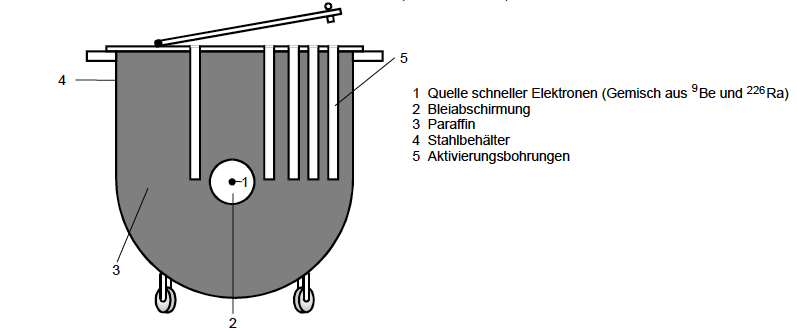
\includegraphics[scale=0.5]{a.PNG}
  \caption{schematischer Aufbau der Neutronenquelle.\cite{Q1}}
  \label{abb1}
\end{figure}
\FloatBarrier
Es ist einfacher, die in einem bestimmten Zeitintervall $\Delta t$ zerfallenen Kerne zu bestimen,
als die ncoh vorhandenen Kerne zu untersuchen. Dies ist begründet darin, dass es geeigente Strahlungsdetektoren
gibt, die bei jedem Zerfall einen elektrischen Puls abgeben, welche deutlich leichter quantifizierbar sind.
Hierbei ist jedoch zu beachten, dass die Wahl des $\Delta t$ gewisse Risiken birgt:
Wird es zu groß gewählt, entsteht ein systematischer Fehler, wird es zu klein gewählt, so entstehen
statistische Fehler.
Die Zahl, der in einem Zeitintervall $\Delta t$ zerfallenen Kerne wird durch folgende Formel
beschrieben:
\FloatBarrier
\begin{align*}
  \label{eq:3}
  N_{\Delta t}(t) &= N(t)~-~N(t~+~\Delta t) \\
  N_{\Delta t}(t) &=N_0\left(1-\symup{exp}(-\lambda \Delta t)\right)\symup{exp}(- \lambda t)\\
\end{align*}
Für die Auswertung des Versuchs von besonderer Bedeutung ist der Zerfall von Rhodium.
Wird der Kern von $\ce{^{103}_{45}Rh}$ aktiviert, so entsteht mit einer Wahrscheinlichkeit
von $\SI{90}{\percent}$, $\ce{^{104}_{45}Rh}$ und mit einer Wahrscheinlichkeit von
$\SI{10}{\percent}$, dessen ernergiereichere Vorstufe
$\ce{^{104i}_{45}Rh}$ . Sie ist, wie bereits erwähnt lediglich eine enrgiereichere
Vorstufe des Rhodiumisotops, die unter Emission eines $\gamma$~-~Quants zu $\ce{^{104}_{45}Rh}$
zerfällt.
Die beiden Zerfälle laufen parallel und mit unterschiedlichen Halbwertszeiten ab. Die Gesamtaktivität
wird durch die Summe beider Zerfälle ausgedrückt.
Nach hinreichend langer Zeit $t^*$ , ist davon auszugehen, dass alle kurzlebigeren
$\ce{^{104i}_{45}Rh}$ - Kerne zerfallen sind und nur noch die stabileren $\ce{^{104}_{45}Rh}$ - Kerne
zerfallen, was sich im Zerfallsdiagramm  \ref{abb2} als eine Gerade darstellen sollte.
\FloatBarrier
\begin{figure}
  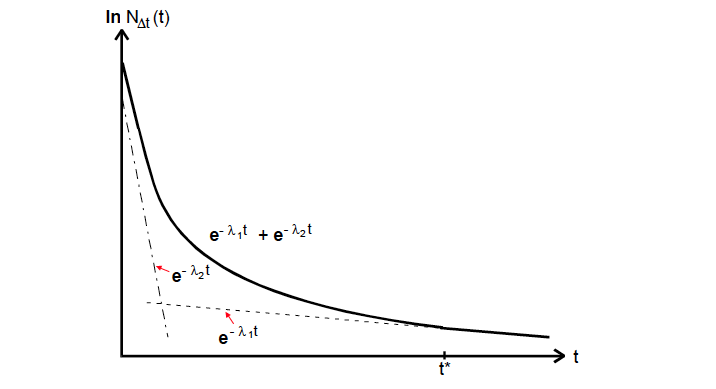
\includegraphics[scale=0.7]{b.PNG}
  \caption{Zerfallskurve eines Präparates mit unterschiedlichen Zerfallskonstanten mit eingezeichnetem $t^*$.\cite{Q1}}
  \label{abb2}
\end{figure}
\FloatBarrier
Es bleibt der Vollständigkeit halber zu erwähnen, dass der im Versuch verwendete
Detektor in der Lage ist , ebenfalls die beim $\ce{^{104i}_{45}Rh}$ - Zerfall frei
werdenden $\gamma$~-~Strahlen aufzunhemen.
Der Anteil dieses Zerfalls ist jedoch als so gering zu betrachten, dass er keinen nennswerten Einfluss
auf die Gesamtbilanz hat und deshalb vernachlässigt werden kann.
Der Zerfall von Rhodium läuft wie folgt ab:
\FloatBarrier
\begin{equation*}
  \ce{^{103}_{45}Rh} + \symup{n} \begin{cases} \ce{ ->[\SI{10}{\percent}]}  \ce{^{104i}_{45}Rh} \ce{->} \ce{^{104}_{45}Rh} +  \ce{$\gamma$} \ce{->} \ce{^{104}_{46}Pd} + \ce{$\beta$-}  + \overline{\nu_{\symup{e}}} \\
  \ce{ ->[\SI{90}{\percent}]} \ce{^{104}_{45}Rh}  \ce{->} \ce{^{104}_{46}Pd} + \ce{$\beta$-}   + \overline{\nu_{\symup{e}}} \end{cases}
\end{equation*}
\FloatBarrier

\section{Durchführung}
Die Messungen werden allesamt mit einem Geiger-Müller-Zählrohr durchgeführt, an den
ein Straghlungsdetektor angeschlossen ist. Der Detektor registriert die auftreffenden
Teilchen, die an einem Verstärkerausgang einen elektrischen Impuls liefern. Der Detektor besitzt
zwei Anzeigevorrichtungen, die periodisch umgeschaltet werden und in denen die Anzahl der während $\Delta t$
stattgefunden Ereignisse angezeigt werden. Ein schematischer Aufbau der Versuchsapparatur ist
in Abbildung \ref{abb3} zu sehen.
\FloatBarrier
\begin{figure}
  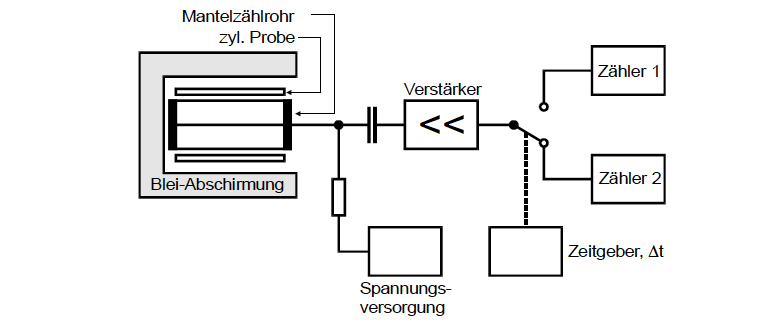
\includegraphics[scale=0.5]{c.PNG}
  \caption{Schematischer Aufbau der Messaparatur.\cite{Q1}}
  \label{abb3}
\end{figure}
\FloatBarrier
Zu Beginn des Versuchs wird die sogenannte Nullrate $N_u$ ermittelt. Die Nullrate ist die
Anzahl der vom Detektor registrierten elektrischen Impulse, die in Abwesenheit einer
radioaktiven Probe gemessen werden können. Sie entsteht zum Beispiel durch Höhenstrahlung.
Hierfür wird die Probenhalterung im Geiger-Müller-Zählrohr leer gelassen und die Zähluhr
auf $\SI{240}{\second}$ gestellt. Der Wert für die stattgefundenen Ereignisse ist leicht abzulesen und wird notiert.
Im Anschluss daran wird ein einfacher Zerfall von Vanadium ($\ce{^{51}_{23}V}$) untersucht. Hierfür wird eine
aktivierte Probe $\ce{^{52}_{23}V}$ in das Geiger-Müller-Zählrohr eingeführt und die
Anzahl der Ereignisse, die während der einzelnen Zeitintervalle ($\Delta t = \SI{20}{\second}$) stattfinden, notiert.
Die Länge für $\Delta t$ und die Gesamtdauer der Messung kann einer am Versuchsort
vorligenden Tabelle entnommen werden.
Zum Schluss wird aktiviertes Rhodium auf die gleiche Weise untersucht. Die Dauer
der Messung ($\SI{12}{\minute}$), sowie das geeignete Zeitintervall ($\Delta t = \SI{20}{\second}$) werden auch hier
wieder einer am Versuchsort vorliegenden Tabelle entnommen.


\section{Auswertung}
Im folgenden Versuch werden die Fehler der gemessenen Ausschläge des Geiger-Müller-Zählers immer mit $\sqrt{N}$ berechnet, da diese Messung der Poisson-Verteilung unterliegt.
\subsection{Nullmessung}
Es wurden innerhalb von $t=\SI{240}{\second}$ $N=216$ Ausschläge am Geiger-Müller-Zählrohr gemessen.
Dies entspricht einem Wert von $N_{\symup{null}} = \SI{0,90(6)}{\per\second}$. Der Fehler der Messung wurde mit $\Delta N_{\symup{null}} = \frac{\sqrt{N}}{t}$
berechnet.

\subsection{Vanadium}
Die Messwerte und die berechneten Größen sind in Tabelle \ref{tab:1} zu finden. Zur Messung der Zerfallskonstante von Vanadium muss zunächst die Untergrundstrahlung
von den gemessenen Ausschlägen des Geiger-Müller-Zählrohrs abgezogen werden.
Die Untergrundstrahlung $N_U$ ist für ein Zeitintervall der Länge $\Delta t = \SI{30}{\second}$:
\begin{equation*}
  N_U = N_{\symup{null}} \cdot \Delta t = \SI{27,0(18)}{\second}
\end{equation*}
Daraus folgt für die Ausschläge ohne Untergundstrahlung
\begin{align}
  N_{\symup{\Delta t}} &= N_{\symup{\Delta t \, mit \, U}} - N_U
  \label{eq:Untergrundsubtraktion} \\
  \Delta N_{\symup{\Delta t}} &= \sqrt{(\Delta N_{\symup{\Delta t \, mit \, U}})²+(\Delta N_U)²}
  \label{eq:UntergrundsubtraktionFehler}
\end{align}
Durch das Zerfallsgesetz
\begin{equation*}
    N_{\symup{\Delta t}} = N_{\symup{0}} \symup{e}^{- \lambda t}
\end{equation*}
kann nun eine Aussage über die Zerfallskonstante $\lambda$ getroffen werden, indem eine lineare Regression der Form
\begin{equation*}
  \symup{ln}(N_{\symup{\Delta t}}(t)) = a_1 \cdot t + b_1
\end{equation*}
durchgeführt wird. Diese Regression (siehe Abbildung \ref{plot1}) liefert die Werte für $a_1$ und $b_1$
\begin{align*}
  a_1 &= \SI{-3,47(26)e-3}{\per\second} \\
  b_1 &= \num{5,67(16)}
\end{align*}
Durch Vergleich mit dem Zerfallsgesetz folgt für die Zerfallskonstante $\lambda$ und die Konstante $N_0$
\begin{align*}
  \lambda_{\symup{Vanadium}} &= -a_1 = \SI{3,47(26)e-3}{\per\second} \\
  N_{\symup{0 \, Vanadium}} &= \symup{e}^{b_1} = \num{290(46)} \ ,
\end{align*}
wobei der Fehler von $N_0$ mit
\begin{equation}
  \Delta N_0 = \symup{e}^{b_1} \cdot \Delta b_1
  \label{eq:bFehler}
\end{equation}
berechnet wurde. Daraus folgt für die Halbwertszeit $T_{\symup{1/2}}$ für Vanadium nach der Formel
\begin{align}
  T_{\symup{1/2}} = \frac{-\symup{ln(2)}}{\lambda}
  \label{Halbwertszeit} \\
  \Delta T_{\symup{1/2}} = \frac{\symup{ln(2)}}{\lambda²} \cdot \Delta \lambda
  \label{HalbwertszeitFehler}
\end{align}
\begin{equation*}
  T_{\symup{1/2 \, Vanadium}} = \SI{200(15)}{\second}
\end{equation*}
\begin{figure}
  \centering
  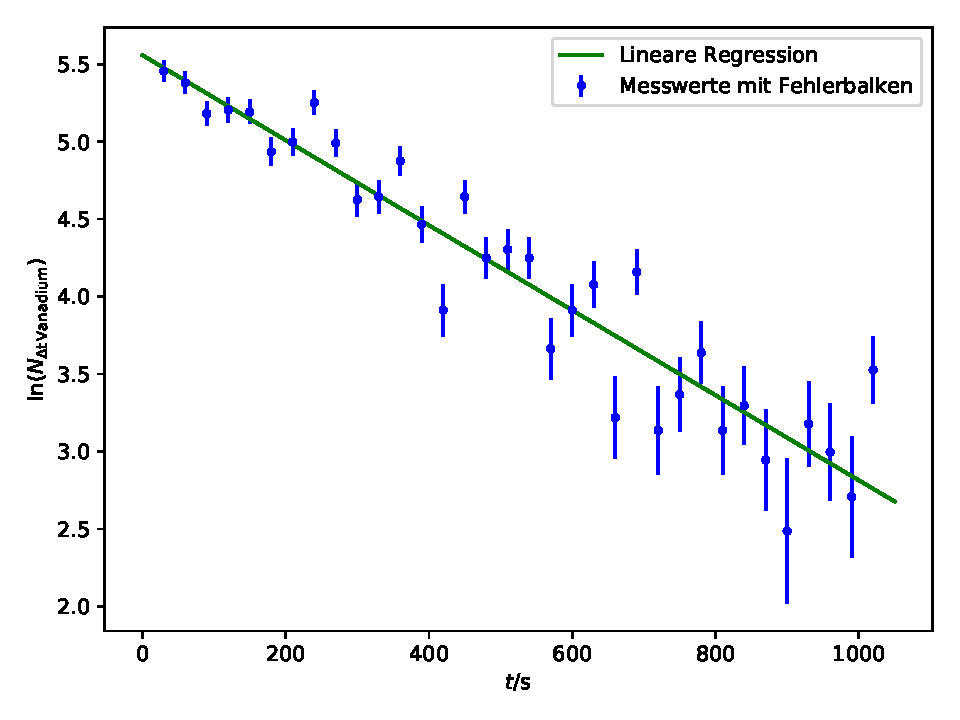
\includegraphics[scale=0.7]{Vanadium.pdf}
  \caption{Messwerte und lineare Regression von Vanadium: Zeit $t$, Anzahl der Ausschläge ohne Untergrundstrahlung $N_{\symup{\Delta t \, Vanadium}}$.}
  \label{plot1}
\end{figure}

\begin{table}[H]
  \centering
  \caption{Messwerte Vanadium: Zeit $t$, Anzahl der Ausschläge des Geiger-Müller-Zählrohrs $N_{\symup{\Delta t \, mit\, U}}$, Anzahl der Ausschläge ohne Untergrundstrahlung $N_{\symup{\Delta t \, Vanadium}}$.}
  \label{tab:1}
  \begin{tabular}{c c c c}
    \toprule
    $t$ / \si{\second} & $N_{\symup{\Delta t \, mit \, U}}$ / Anzahl/\SI{20}{\second} & $N_{\symup{\Delta t \, Vanadium}}$ / Anzahl/\SI{20}{\second} & ln($N_{\symup{\Delta t \, Vanadium}}$)\\
    \midrule
    30 & 252,00 \pm 15,88 & 225,00 \pm 15,98 & 5,42 \pm 0,07 \\
    60 & 235,00 \pm 15,33 & 208,00 \pm 15,44 & 5,34 \pm 0,07 \\
    90 & 196,00 \pm 14,00 & 169,00 \pm 14,12 & 5,13 \pm 0,08 \\
    120 & 200,00 \pm 14,14 & 173,00 \pm 14,26 & 5,15 \pm 0,08 \\
    150 & 198,00 \pm 14,07 & 171,00 \pm 14,19 & 5,14 \pm 0,08 \\
    180 & 157,00 \pm 12,53 & 130,00 \pm 12,66 & 4,87 \pm 0,10 \\
    210 & 166,00 \pm 12,88 & 139,00 \pm 13,01 & 4,93 \pm 0,09 \\
    240 & 209,00 \pm 14,46 & 182,00 \pm 14,57 & 5,20 \pm 0,08 \\
    270 & 165,00 \pm 12,85 & 138,00 \pm 12,98 & 4,93 \pm 0,09 \\
    300 & 120,00 \pm 10,95 & 93,00 \pm 11,11 & 4,53 \pm 0,12 \\
    330 & 122,00 \pm 11,04 & 95,00 \pm 11,20 & 4,55 \pm 0,12 \\
    360 & 149,00 \pm 12,21 & 122,00 \pm 12,34 & 4,80 \pm 0,10 \\
    390 & 105,00 \pm 10,25 & 78,00 \pm 10,41 & 4,36 \pm 0,13 \\
    420 & 68,00 \pm 8,25 & 41,00 \pm 8,45 & 3,71 \pm 0,21 \\
    450 & 122,00 \pm 11,04 & 95,00 \pm 11,20 & 4,55 \pm 0,12 \\
    480 & 88,00 \pm 9,38 & 61,00 \pm 9,56 & 4,11 \pm 0,16 \\
    510 & 92,00 \pm 9,59 & 65,00 \pm 9,77 & 4,17 \pm 0,15 \\
    540 & 88,00 \pm 9,38 & 61,00 \pm 9,56 & 4,11 \pm 0,16 \\
    570 & 57,00 \pm 7,55 & 30,00 \pm 7,77 & 3,40 \pm 0,26 \\
    600 & 68,00 \pm 8,25 & 41,00 \pm 8,45 & 3,71 \pm 0,21 \\
    630 & 77,00 \pm 8,78 & 50,00 \pm 8,96 & 3,91 \pm 0,18 \\
    660 & 43,00 \pm 6,56 & 16,00 \pm 6,81 & 2,77 \pm 0,43 \\
    690 & 82,00 \pm 9,05 & 55,00 \pm 9,24 & 4,01 \pm 0,17 \\
    720 & 41,00 \pm 6,40 & 14,00 \pm 6,66 & 2,64 \pm 0,48 \\
    750 & 47,00 \pm 6,86 & 20,00 \pm 7,10 & 3,00 \pm 0,35 \\
    780 & 56,00 \pm 7,48 & 29,00 \pm 7,71 & 3,37 \pm 0,27 \\
    810 & 41,00 \pm 6,40 & 14,00 \pm 6,66 & 2,64 \pm 0,48 \\
    840 & 45,00 \pm 6,71 & 18,00 \pm 6,96 & 2,89 \pm 0,39 \\
    870 & 37,00 \pm 6,08 & 10,00 \pm 6,35 & 2,30 \pm 0,64 \\
    900 & 30,00 \pm 5,48 & 3,00 \pm 5,78 & 1,10 \pm 1,93 \\
    930 & 42,00 \pm 6,48 & 15,00 \pm 6,74 & 2,71 \pm 0,45 \\
    960 & 38,00 \pm 6,16 & 11,00 \pm 6,43 & 2,40 \pm 0,58 \\
    990 & 33,00 \pm 5,75 & 6,00 \pm 6,03 & 1,79 \pm 1,00 \\
    1020 & 52,00 \pm 7,21 & 25,00 \pm 7,44 & 3,22 \pm 0,30 \\
    \bottomrule
  \end{tabular}
\end{table}

\subsection{Rhodium}
Zunächst muss bei dieser Messung erneut die Untergrundstrahlung abgezogen werden. Da hier ein anderen Zeitintervall zur Messung gewählt wurde ist nun $\Delta t = \SI{20}{\second}$.
Di Untergrundstrahlung $N_U = N_{\symup{null}} \cdot \Delta t = \SI{18.0(12)}{\second} $ muss von der Messung, mit Hilfe von Gleichung \eqref{eq:Untergrundsubtraktion},
abgezogen werden, da diese für den Zerfall von Rhodium keine Rolle spielt. Der Fehler wurde mit Gleichung \eqref{eq:UntergrundsubtraktionFehler} berechnet.

Die Halbwertszeiten von Rhodium zu berechnen ist nicht ganz so einfach wie die von Vanadium, denn hier finden zwei Zerfälle gleichzeitig statt.
Da einer der beiden Zerfälle aber viel langlebiger ist als der andere, kann nach einer Zeit $t^*$ davon ausgegangen werden, dass nurnoch der langsamere
Zerfall eine Rolle spielt, für diesen Fall $t \geq t^*$ gilt
\begin{equation*}
  N_{\symup{\Delta t \, gesamt}} = N_{\symup{0,1}} \symup{e}^{- \lambda_1 t} + N_{\symup{0,2}} \symup{e}^{- \lambda_2 t} \approx N_{\symup{0,2}} \symup{e}^{- \lambda_2 t}
\end{equation*}
wobei der schnelle Zerfall durch den Index 1 und der langsamere Zerfall durch den Index 2 beschrieben wird.
Durch Betrachtung der Abbildung \ref{plot2} kann man in etwa ablesen, ab wann die Messwerte eine Gerade bilden, in unserer Messung war dies ab $t^* =\SI{220}{\second} $ der Fall.
Nun kann für die Messwerte $t \geq t $ eine lineare Regression der Form
\begin{equation*}
  \symup{ln}(N_{\symup{\Delta t \, 2}}(t)) = a_2  t + b_2
\end{equation*}
durchgeführt werden, diese liefert die Werte für die Steigung $a_2$ und den Y-Achsenabschnitt $b_2$
\begin{align*}
  a_2 &= \SI{-2,70(29)e-3}{\per\second} \\
  b_2 &= \num{5,34(14)}
\end{align*}
Aus dem Vergleich der Regressionsfunktion und der Zerfallsfunktion kann man die Zerfallskonstante $\lambda_2$ und die Konstante $N_{\symup{0,2}}$ berechnen
\begin{align*}
  \lambda_{\symup{2}} &= -a_2 = \SI{2,70(29)e-3}{\per\second} \\
  N_{\symup{0,2}} &= \symup{e}^{b_2} = \num{208(30)} \ \ .
\end{align*}
Der Fehler wurde mittels Gleichung \eqref{eq:bFehler} bestimmt. Mit der Formel \eqref{Halbwertszeit} und \eqref{HalbwertszeitFehler} lässt sich nun die Halbwertszeit des langsamen Zerfalls berechnen
\begin{equation*}
  T_{\symup{1/2, \, 2 \, , Rhodium}} = \SI{257(28)}{\second}
\end{equation*}
Da man aus den vorherigen Berechnungen die Zerfallsfunktion des langsamen Zerfalls kennt, kann man diese nun von dem gesamten Zerfall abziehen und erhält
nurnoch die Werte des schnellen Zerfalls:
\begin{equation*}
  N_{\symup{\Delta t \, 1}}= N_{\symup{\Delta t \, gesamt}} - N_{\symup{0,2}} \symup{e}^{- \lambda_2 t} = N_{\symup{0,1}} \symup{e}^{- \lambda_1 t}
\end{equation*}
Der Fehler wurde mit der folgenden Formel bestimmt
\begin{equation*}
  \Delta N_{\symup{\Delta t,1}} = \sqrt{(\Delta N_{\symup{0,2}} \cdot \symup{e}^{-\lambda_2 t})²+( N_{\symup{0,2}} t \cdot \Delta \lambda_2 \cdot \symup{e}^{-\lambda_2 t} )²+(\Delta N_{\symup{\Delta t, gesamt}})²}.
\end{equation*}
Mit den Werten von $N_{\symup{\Delta t \, 1}}$ lässt sich somit eine lineare Regression durchführen. Um zu vermeiden, dass die berechneten Werte
kleiner als Null werden, muss eine Grenze $t_{\symup{max}}$ gesetzt werden. Hier haben wir die maximale Zeit bei
$t_{\symup{max}} = \SI{160}{\second}$ angesetzt. Nun kann für $ t \leq t_{\symup{max}}$ eine lineare Regression der Form
\begin{equation*}
  \symup{ln}(N_{\symup{\Delta t \, 1}}(t)) = a_3  t + b_3
\end{equation*}
durchgeführt werden. Diese Regression liefert die Werte für die Steigung und den y-Achsenabschnitt
\begin{align*}
  a_3 &= \SI{-2,06(9)e-2}{\per\second} \\
  b_3 &= \num{7,31(9)} \ .
\end{align*}
Der Vergleich zwischen der linearen Regression und der Zerfallsfunktion liefert die Werte für die Zerfallskonstante $\lambda_{\symup{1}}$ und die Konstante $N_{\symup{0,1}}$
\begin{align*}
  \lambda_{\symup{1}} &= -a_3 = \SI{2,06(9)e-2}{\per\second} \\
  N_{\symup{0,1}} &= \symup{e}^{b_3} = \num{1490(130)} \ .
\end{align*}
Der Fehler wurde mit der Gleichung \eqref{eq:bFehler} berechnet. Durch die Gleichung \eqref{Halbwertszeit} und \eqref{HalbwertszeitFehler} lässt sich die Halbwertszeit für den schnellen Zerfall berechnen
\begin{equation*}
  T_{\symup{1/2, \, 1 \, , Rhodium}} = \SI{33,7(14)}{\second}
\end{equation*}
\newpage
\begin{figure}
  \centering
  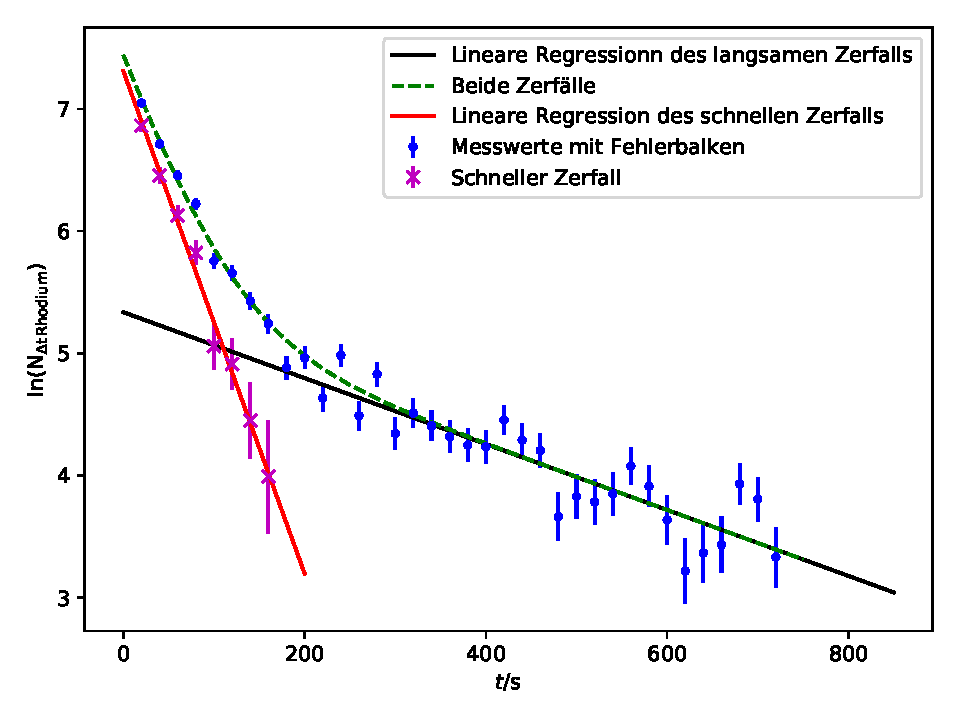
\includegraphics[scale=0.7]{Rhodium2.pdf}
  \caption{Messwerte und lineare Regression von Rhodium: Zeit $t$, Anzahl der Ausschläge ohne Untergrundstrahlung $N_{\symup{\Delta t \, Rhodium}}$.}
  \label{plot2}
\end{figure}
\begin{table}
  \centering
  \caption{Messwerte für die Regression des schnellen Zerfalls von Rhodium.}
  \label{tab:3}
  \begin{tabular}{c c c c}
    \toprule
    $t$ / \si{\second} & $N_{\symup{\Delta t \, mit U }}$ / Anzahl/\SI{20}{\second} & $N_{\symup{\Delta t \, ,1,  Rhodium}}$ / Anzahl/\SI{20}{\second} & ln($N_{\symup{\Delta t \, ,1,Rhodium}}$)\\
    \midrule
    20,00 & 116,.00 \pm 34,18 & 953,15 \pm 44,37 & 6,86 \pm 0,05 \\
    40,00 & 840,00 \pm 28,98 & 635,49 \pm 39,53 & 6,45 \pm 0,06 \\
    60,00 & 653,00 \pm 25,55 & 458,28 \pm 36,15 & 6,13 \pm 0,08 \\
    80,00 & 523,00 \pm 22,87 & 337,56 \pm 33,42 & 5,82 \pm 0,10 \\
    100,00 & 334,00 \pm 18,28 & 157,35 \pm 29,58 & 5,06 \pm 0,19 \\
    120,00 & 304,00 \pm 17,44 & 135,68 \pm 28,25 & 4,91 \pm 0,21 \\
    140,00 & 246,00 \pm 15,68 & 85,58 \pm 26,43 & 4,45 \pm 0,31 \\
    160,00 & 207,00 \pm 14,39 & 54,05 \pm 24,96 & 3,99 \pm 0,46 \\
    \bottomrule
  \end{tabular}
\end{table}
\newpage
\begin{table}
  \centering
  \caption{Messwerte Rhodium: Zeit $t$, Anzahl der Ausschläge des Geiger-Müller-Zählrohrs $N_{\symup{\Delta t \, mit \, U}}$, Anzahl der Ausschläge ohne Untergrundstrahlung $N_{\symup{\Delta t \, Rhodium}}$.}
  \label{tab:3}
  \begin{tabular}{c c c c}
    \toprule
    $t$ / \si{\second} & $N_{\symup{\Delta t \, mit U}}$ / Anzahl/\SI{20}{\second} & $N_{\symup{\Delta t \, Rhodium}}$ / Anzahl/\SI{20}{\second} & ln($N_{\symup{\Delta t \, Rhodium}}$)\\
    \midrule
    20 & 1168,00 \pm 34,18 & 1150,00 \pm 34,20 & 7,05 \pm 0,03 \\
    40 & 840,00 \pm 28,98 & 822,00 \pm 29,01 & 6,71 \pm 0,04 \\
    60 & 653,00 \pm 25,55 & 635,00 \pm 25,58 & 6,45 \pm 0,04 \\
    80 & 523,00 \pm 22,87 & 505,00 \pm 22,90 & 6,22 \pm 0,04 \\
    100 & 334,00 \pm 18,28 & 316,00 \pm 18,32 & 5,76 \pm 0,06 \\
    120 & 304,00 \pm 17,44 & 286,00 \pm 17,48 & 5,66 \pm 0,06 \\
    140 & 246,00 \pm 15,68 & 228,00 \pm 15,73 & 5,43 \pm 0,07 \\
    160 & 207,00 \pm 14,39 & 189,00 \pm 14,44 & 5,24 \pm 0,08 \\
    180 & 150,00 \pm 12,25 & 132,00 \pm 12,31 & 4,88 \pm 0,09 \\
    200 & 161,00 \pm 12,69 & 143,00 \pm 12,75 & 4,96 \pm 0,09 \\
    220 & 121,00 \pm 11,00 & 103,00 \pm 11,07 & 4,63 \pm 0,11 \\
    240 & 164,00 \pm 12,81 & 146,00 \pm 12,87 & 4,98 \pm 0,09 \\
    260 & 107,00 \pm 10,34 & 89,00 \pm 10,42 & 4,49 \pm 0,12 \\
    280 & 143,00 \pm 11,96 & 125,00 \pm 12,02 & 4,83 \pm 0,10 \\
    300 & 95,00 \pm 9,75 & 77,00 \pm 9,82 & 4,34 \pm 0,13 \\
    320 & 109,00 \pm 10,44 & 91,00 \pm 10,51 & 4,51 \pm 0,12 \\
    340 & 100,00 \pm 10,00 & 82,00 \pm 10,07 & 4,41 \pm 0,12 \\
    360 & 93,00 \pm 9,64 & 75,00 \pm 9,72 & 4,32 \pm 0,13 \\
    380 & 88,00 \pm 9,38 & 70,00 \pm 9,46 & 4,25 \pm 0,14 \\
    400 & 87,00 \pm 9,33 & 69,00 \pm 9,41 & 4,23 \pm 0,14 \\
    420 & 104,00 \pm 10,20 & 86,00 \pm 10,27 & 4,45 \pm 0,12 \\
    440 & 91,00 \pm 9,54 & 73,00 \pm 9,62 & 4,29 \pm 0,13 \\
    460 & 85,00 \pm 9,22 & 67,00 \pm 9,30 & 4,21 \pm 0,14 \\
    480 & 57,00 \pm 7,55 & 39,00 \pm 7,65 & 3,66 \pm 0,20 \\
    500 & 64,00 \pm 8,00 & 46,00 \pm 8,09 & 3,83 \pm 0,18 \\
    520 & 62,00 \pm 7,87 & 44,00 \pm 7,97 & 3,78 \pm 0,18 \\
    540 & 65,00 \pm 8,06 & 47,00 \pm 8,15 & 3,85 \pm 0,17 \\
    560 & 77,00 \pm 8,78 & 59,00 \pm 8,86 & 4,08 \pm 0,15 \\
    580 & 68,00 \pm 8,25 & 50,00 \pm 8,34 & 3,91 \pm 0,17 \\
    600 & 56,00 \pm 7,48 & 38,00 \pm 7,58 & 3,64 \pm 0,20 \\
    620 & 43,00 \pm 6,56 & 25,00 \pm 6,67 & 3,22 \pm 0,27 \\
    640 & 47,00 \pm 6,86 & 29,00 \pm 6,96 & 3,37 \pm 0,24 \\
    660 & 49,00 \pm 7,00 & 31,00 \pm 7,11 & 3,43 \pm 0,23 \\
    680 & 69,00 \pm 8,31 & 51,00 \pm 8,40 & 3,93 \pm 0,17 \\
    700 & 63,00 \pm 7,94 & 45,00 \pm 8,03 & 3,81 \pm 0,18 \\
    720 & 46,00 \pm 6,78 & 28,00 \pm 6,89 & 3,33 \pm 0,25 \\
    \bottomrule
  \end{tabular}
\end{table}


\section{Diskussion}
Die berechneten Halbwertszeiten und deren Literaturwerte sind in Tabelle \ref{tab:diskussion} zusammengefasst.
\begin{table}
  \centering
  \caption{Vergleich: berechnete Werte und Literaturwerte für die Halbwertszeiten. \cite{Q2} \cite{Q3}}
  \label{tab:diskussion}
  \begin{tabular}{c |c c c}
    \toprule
    & berechnete Halbwertszeit & Literaturwert & Abweichung \\
    & $T_{\symup{1/2}}$ / \si{\second} & $T_{\symup{1/2, Literatur}}$ / \si{\second} & $p$ / \si{\percent} \\
    \midrule
    Vanadium & 200 \pm 15 & 224,6 & 10,95 \\
    Rhodium 1 & 33,7 \pm 14 & 42,3 & 20,33 \\
    Rhodium 2 & 257 \pm 28 & 260,4 & 1,31 \\
    \bottomrule
  \end{tabular}
\end{table}
Die Literaturwerte der Halbwertszeiten von Rhodium liegen in dem von uns berechneten Fehlerintervall. Die berechnete Halbwertszeit von Vanadium weicht
um etwa \SI{10}{\percent} von dem Literaturwert ab. Eine Fehlerquelle die zu solchen Abweichungen führen kann, ist die Nullmessung. Diese konnte nur für
eine Zeit von $t=\SI{240}{\second}$ durchgeführt werden, da der automatische Zähler in hohen Zeitintervallen nicht gemessen hat. Diese zu kurze Messung
der Untergrundstrahlung führt zu statistischen Fehlern für $N_U$ und somit weiterführend für die ganze Berechnung der Halbwertszeiten.

Bei Rhodium lässt sich außerdem berechnen, mit welcher Wahrscheinlichkeit welcher der beiden Zerfälle stattfindet. Durch die
Konstanten $N_{0,1}, N_{0,2}$, welche die Zerfallenen Kerne beschreiben, kann man den Anteil der zerfallenen Kerne des langsamen Zerfalls berechnen:
\begin{equation*}
  p = \frac{N_{\symup{0,2, Rhodium}}}{N_{\symup{0,1, Rhodium}}+N_{\symup{0,2, Rhodium}}} \approx \SI{12,25}{\percent}
\end{equation*}
Dieser Anteil stimmt ungefähr mit dem Anteil aus der Literatur von $p_{\symup{Literatur}} \approx \SI{10}{\percent}$ überein(\cite{Q1}).

\nocite{*}
\printbibliography
